\documentclass[12pt]{article}

\usepackage{sbc-template}

\usepackage{graphicx,url}

\usepackage[brazil]{babel}   
%\usepackage[latin1]{inputenc}  
\usepackage[utf8]{inputenc}  
% UTF-8 encoding is recommended by ShareLaTex
\usepackage{verbatim}
\usepackage{listings}
\usepackage{xcolor}

\definecolor{verde}{rgb}{0,0.5,0}

%para customizar o código (ver https://en.wikibooks.org/wiki/LaTeX/Source_Code_Listings)
\lstset{language=C, %defina a linguagem usada no trabalho
              belowcaptionskip=1\baselineskip,
                breaklines=true,
                frame=false,
                xleftmargin=\parindent,
                showstringspaces=false,
                basicstyle=\footnotesize\ttfamily,
                keywordstyle=\bfseries\color{green!40!black},
                commentstyle=\itshape\color{purple!40!black},
                identifierstyle=\color{blue},
                stringstyle=\color{orange},
                numbers=left,
            }

\sloppy

\title{Proyecto social: Acercamiento a la comunidad a través de la programación. }

\author{Alejandro Iabin Arteaga Hernández\\ \href{iabin@ciencias.unam.mx}} 

\begin{document} 

\maketitle

\begin{resumo}
  Propongo curso de computación básica, en instalaciones de la delegación, me ofrezco como profesor voluntario, 
  soy estudiante de 4to semestre de la carrera Ciencias de la computación en la facultad de ciencias de la 
  UNAM, el curso propuesto dura 20 horas, 2 horas semanales, pero pueden ser más o menos.
  
\end{resumo}


\section{Introducción}

La importancia de las computadoras es cada día mayor, por eso es indispensable que todos los individuos sean capaces de manipularlas con comodidad y realizar tareas cotidianas, asi como tareas en el ámbito laboral, debido a que los individuos con mejor manejo del computador tiene mejor probabilidad de encontrar un empleo mejor remunerado.\\     Lamentablemente los cursos suelen ser caros, y un gran número de personas no pueden costearlos. Por eso mismo, propongo este curso, que va dirigido al público que cuente con muy poco o ningún manejo de la computadora   .


\section{Datos técnicos} \label{sec:firstpage}

\textbf{\textit{Requisitos que pido para el curso:}}\\
Lo deseable sería salón con computadoras, no importa que tan viejas sean, solo necesitan acceso a internet. 
    Si no se pudiese, con un salón y un proyector es suficiente \\ \\
    Las clases serían en sábado o domingo, a la hora que se pueda, a mi me gustaría de 2 a 4, pero no estoy seguro de cual sea el horario mas accesible para la gente.

\section{Metodologia}

Descreve os métodos e técnicas utilizados na pesquisa

\subsection{Sobre seções e parágrafos}

Os títulos das seções devem estar em negrito, fonte 13pt, alinhados a esquerda. A linha do título da seção deve possuir 12pts de espaçamento antes do seu início. A numeração das seções é opcional, embora recomendado. O primeiro parágrafo de cada seção não deve ser tabulado, enquanto que as primeiras linhas dos parágrafos subsequentes devem ser tabulados em 1.27 cm.

Os títulos das subseções devem estar em negrito, 12pt, alinhados a esquerda.


\section{Análise dos dados}\label{sec:analisedosdados}

Nesta seção, o aluno descreve o efetivo procedimento metodológico adotado e aponta os resultados da pesquisa. Na análise de dados, é  aconselhável o uso de tabelas, figuras, linhas de códigos etc para representar os resultados do estudo.

As Tabelas, Quadros e Figuras, assim como as legendas de Tabelas, Quadros e Figuras devem estar centralizadas se conterem apenas em uma linha (Figura~\ref{fig:figura1}), caso contrário devem estar tabuladas em 0.8cm em ambas as margens, como mostra a Figura~\ref{fig:figura2}. 

\begin{figure}[ht]
\centering
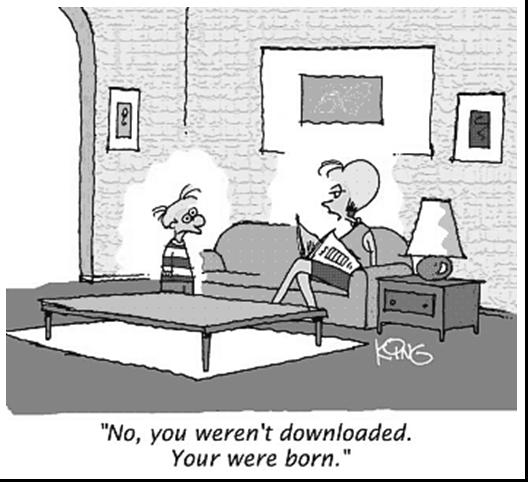
\includegraphics[width=.3\textwidth]{fig1.jpg}
\caption{Exemplo de figura}
\label{fig:figura1}
\end{figure}

As legendas devem ser escritas na fonte “Helvetica”, Tamanho 10pts, negrito, com espaço de 6pts antes e depois de cada legenda. Sempre que possível, procure colocar a figura delimitada por um quadro (Figura~\ref{fig:figura1} e Figura~\ref{fig:figura2})

\begin{figure}[!ht]
\centering
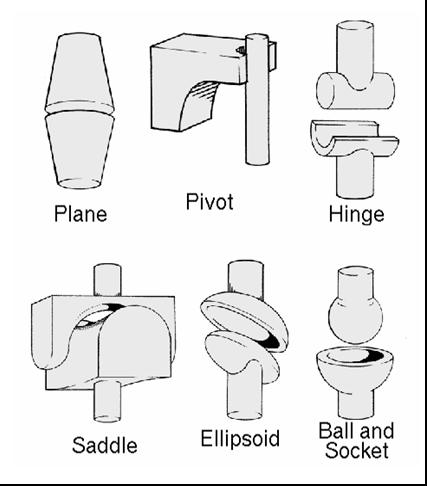
\includegraphics[width=.2\textwidth]{fig2.jpg}
\caption{Essa figura foi referenciada na Seção~\ref{sec:analisedosdados}.}
\caption{Fonte: SBC.}
\label{fig:figura2}
\end{figure}

Em tabelas, tente evitar o uso de fundos coloridos ou preenchidos, assim como linhas duplas na borda, ou linhas desnecessárias. Quando \cite{knuth:84} relatar dados empíricos, não faça uso de mais dígitos decimais do que o necessário. A legenda da tabela deve ser colocada antes da tabela (veja Tabela 1) e a fonte usada na legenda deve ser Helvetica, tamanho 10pts, negrito, com 6pts de espaço antes e depois de cada legenda.

\begin{table}[!ht]
\centering
\caption{Exemplo de tabela de 3 colunas e 2 linhas}
\label{tab:exTable1}
\smallskip
\begin{tabular}{l c c}
\hline
& Value 1 & Value 2\\[0.5ex]
\hline
&&\\[-2ex]
Case 1 & 1.0 $\pm$ 0.1 & 1.75$\times$10$^{-5}$ $\pm$ 5$\times$10$^{-7}$\\[0.5ex]
\hline
&&\\[-2ex]
Case 2 & 0.003(1) & 100.0\\[0.5ex]
\hline
\end{tabular}
\end{table}

\subsection{Código fonte}
A inserção de código fonte deve ser por meio

\begin{lstlisting}

int main(){
  int a,b,c;
  float x;
  printf("informe o tamanho do lado do quadrado");
  scanf("%d", &a);
  printf("A area do quadrado %d", b=area(a));
  printf("Duas vezes o valor do lado do quadrado %d", c=aumenta(a));

\end{lstlisting}



\section{Considerações Finais}

Referências bibliográficas devem ser utilizadas dentro de um estilo uniforme e não ambíguo. A SBC sugere os seguintes formatos para referências: \cite{knuth:84}, \cite{boulic:91}, e \cite{smith:99}.

\bibliographystyle{sbc}
\bibliography{sbc-template}

\end{document}
